\addcontentsline{toc}{subsubsection}{Illustrations: Applications of Integration}
\vbtitle{Illustrations: Applications of Integration}
\BgThispage
\begin{enumerate}
    \item Find the area of a circle of radius $r$.
    \begin{solution}
        \begin{center}
            \begin{tikzpicture}
                \tzcoor*(0, 0)(O)
                \tzcircle(O)(2)
                \tzring[pattern=north east lines](O)(1)(O)(1.2)
                \tzline[->](O)(30:1){$x$}[ma]
                \tzline[<-]($(O)+(30:1.2)$)(30:1.7){$d\!x$}[ma]
                \tzrectangle[pattern=north east lines](-pi, -2.5)(pi, -2.3)
                \tzline[|<->|](-pi, -2.7)(pi, -2.7){$2\pi x$}[mb]
                \tzline[|<-|]<0.25, 0>(pi, -2.5)(pi, -2.3){$d\!x$}[mr]
            \end{tikzpicture}
        \end{center}
        \begin{align*}
            \intertext{Consider a circle of radius $r$.}
            % A &= \pi r^2\\
            \intertext{To find the area of the circle, we can divide the circle into thin rings of width $d\!x$. If we expand the ring, it will look like a rectangle with width $2\pi x$ and height $d\!x$.}
            \intertext{The area of this thin differential ring will be $dA$.}
            dA &= 2\pi x dx\\
            \intertext{If we sum up the areas of all these rings, we get the area of the circle.}
            A &= \int_0^r dA\\
            &= \int_0^r 2\pi x dx\\
            &= 2\pi \int_0^r x dx\\
            &= 2\pi \left[\frac{x^2}{2}\right]_0^r\\
            \Aboxed{A &= \pi r^2}
        \end{align*}
        \vbstarednote{\textcolor{black}{Whatever the geometry of the shape we deal with, if we can think that in terms of differential elements, we can find the area/volume/other quantity  using integration. Here, differential ring is the differential element for the circle. There can be multiple ways to think about the differential element. Let's try this circle from another perspective.} This time we can assume the differential element as a sector with central angle $d\!\theta$. If we integrate the area of all these sectors, we will get the area of the circle.}

        \begin{multicols}{2}
            \begin{align*}
                % \intertext{This time, consider a sector of the circle with central angle $d\!\theta$. The area of this sector will be $dA$.}
                \intertext{As the central angle $d\!\theta$, is small enough, the sector will look like a triangle with base $d\!l=r d\!\theta$ and height $r$.}
                d\!A &= \frac{1}{2} r^2 d\!\theta\\
                \int_0^A d\!A &= \int_0^{2\pi} \frac{1}{2} r^2 d\!\theta\\
                A &= \frac{1}{2} r^2 \int_0^{2\pi} d\!\theta\\
                A &= \frac{1}{2} r^2 \left[\theta\right]_0^{2\pi}\\
                \Aboxed{A &= \pi r^2}
            \end{align*}
            \begin{center}
                \begin{tikzpicture}
                    \tzcoor*(0, 0)(O)
                    \tzcircle(O)(2)  
                    \tzline[->](O)(3, 0)
                    \tzline(O)(30:2)
                    \tzline(O)(40:2)
                    \tzanglemark(2, 0)(O)(30:2){$\theta$}[pos=2]
                    \tzanglemark(30:2)(O)(40:2){$d\!\theta$}[pos=3]
                    \tzarc[|<->|](O)(30:40:2.25){$d\!l$}[ma, sloped]
                    \tzwedge[pattern=north east lines](O)(30:40:2)
                \end{tikzpicture}
            \end{center}
        \end{multicols}
    \end{solution}

\item Find the surface area of a sphere of radius $r$.
    \begin{solution}
        \begin{center}
            \begin{tikzpicture}
                \def\R{2}
                \def\A{37}
                \def\AA{42}
                \tzcoor*(0, 0)(O)
                \tzcircle(O)(\R)
                % \tzellipsering*[blue](O)(1 and 1)(O)(1.5cm)
                % \tzarc[pattern=north east lines, even odd rule](0, 2*sin{\A})(180:360:2*cos{\A} and 0.5)(0, 2*sin{\AA})(180:360:2*cos{\AA} and 0.4)
                \tzarc[pattern=north east lines]"arcone"(0, 2*sin{\A})(180:360:2*cos{\A} and 0.45)
                \tzarc[fill=white]"arctwo"(0, 2*sin{\AA})(180:360:2*cos{\AA} and 0.35)
                \tzarc[dashed]"arctwo"(0, 2*sin{\AA})(0:180:2*cos{\AA} and 0.35)
                \tzline(O)(2*cos{\A}, 2*sin{\A})
                \tzline(O)(2*cos{\AA}, 2*sin{\AA})
                \tzcoor*(0, 2*sin{\A})(O')
                \tzline(O')(2*cos{\A}, 2*sin{\A}){$x$}[ma]
                \tzline(O)(2, 0)
                \tzanglemark(2, 0)(O)(2*cos{\A}, 2*sin{\A}){$\theta$}[pos=2]
                \tzrectangle[pattern=north east lines](-pi, -2.5)(pi, -2.3)
                \tzline[|<->|](-pi, -2.7)(pi, -2.7){$2\pi x$}[mb]
                \tzline[|<-|]<0.25, 0>(pi, -2.5)(pi, -2.3){$d\!l$}[mr]
                \tzarc[|<->|](O)(\A:\AA:2.25){$d\!l$}[ma, sloped] 
            \end{tikzpicture}
        \end{center}
        \BgThispage
        \begin{align*}
            \intertext{Again, consider a sphere of radius $r$ and think about how the surface of this sphere can be constructed using some simple geometry. If you take a rectangular thin stripe and try to wrap it around the sphere, it will look like a differential ring. Whole sphere can be covered by these differential rings. Now, our focus should be on finding the area of this differential ring. If we can find the area of this differential ring, we can sum up the areas of all these rings to get the surface area of the sphere.}
            \intertext{The area of this thin differential ring will be $d\!A$.}
            dA &= 2\pi x d\!l\\
            \intertext{You maybe be thinking about how we got this $2\pi x d\!l$. If you think about the differential ring as a rectangle, the width of the rectangle will be $2\pi x$ and the height will be $d\!l$. $x$ is the cos component of radius and $d\!l$ is the length of arc on the curvature of the sphere.}
            x &= r \cos \theta \quad \text{and} \quad d\!l = r d\theta\\
            dA &= 2\pi r \cos \theta r d\theta\\
            \intertext{If we sum up the areas of all these rings, we get the surface area of the sphere.}
            A &= \int_{-\pi/2}^{\pi/2} dA\\
            \intertext{Limits are from $-\pi/2$ to $\pi/2$, $\theta$ is position of the ring on the sphere. If we move the ring down to the bottom of the sphere, $\theta$ will be $-\pi/2$ and if we move it to the top of the sphere, $\theta$ will be $\pi/2$.}
            &= \int_{-\pi/2}^{\pi/2} 2\pi r^2 \cos \theta d\theta\\
            &= 2\pi r^2 \int_{-\pi/2}^{\pi/2} \cos \theta d\theta\\
            &= 2\pi r^2 \left[\sin \theta\right]_{-\pi/2}^{\pi/2}\\
            \Aboxed{A &= 4\pi r^2}
        \end{align*}
    \end{solution}
    

    \item Find the volume of a sphere of radius $r$.
        \begin{solution}
            \begin{align*}
                \intertext{Try yourself.}
            \end{align*}
            \vbstarednote{You can assume the differential element as a disc or even simpler as a thin spherical shell.}
        \end{solution}

    \item Find the area of the region bounded by $y=x^2$, $x=1$, $x=2$ and $y=0$.
        \begin{solution}
            \begin{center}
                \begin{tikzpicture}
                    \tzaxes(-0.25, -0.25)(6, 4){$x$}{$y$}
                    \def\Fn{0.3*\x*\x}
                    \tzfn{\Fn}[0:3.5]{$y=x^2$}[r]
                    \tzfnarea*[pattern=north east lines, opacity=0.8]{\Fn}[2:2.25]
                    \tzvXpoint*{Fn}(2, 0)(A)
                    \tzvXpoint*{Fn}(2.25, 0)(B)
                    \tzline(2, 0)(A)
                    \tzline(2.25, 0)(B)
                    \tzline[|->](2, -0.5)(2.25, -0.5){$d\!x$}[mb]
                    \tzline[|->](0, -0.5)(2, -0.5){$x$}[mb]
                \end{tikzpicture}
            \end{center}
            \begin{align*}
                \intertext{To find the area of this region, we can divide the region into thin rectangles of width $d\!x$ and height determined by the function value $x^2$ at that point.}
                \intertext{The area of this thin differential rectangle will be $dA$.}
                dA &= x^2 dx\\
                \intertext{If we sum up the areas of all these rectangles, we get the area of the region.}
                A &= \int_1^2 dA\\
                &= \int_1^2 x^2 dx\\
                &= \left[\frac{x^3}{3}\right]_1^2\\
                \Aboxed{A &= \frac{7}{3}}
            \end{align*}
        \end{solution}
\BgThispage
        \item The linear mass density (mass per unit length) $\lambda$ of rod $AB$ varies with $\theta$ according as \[ \lambda(\theta) = a\theta, \quad a>0 \]Find mass of the rod.
        \begin{center}
            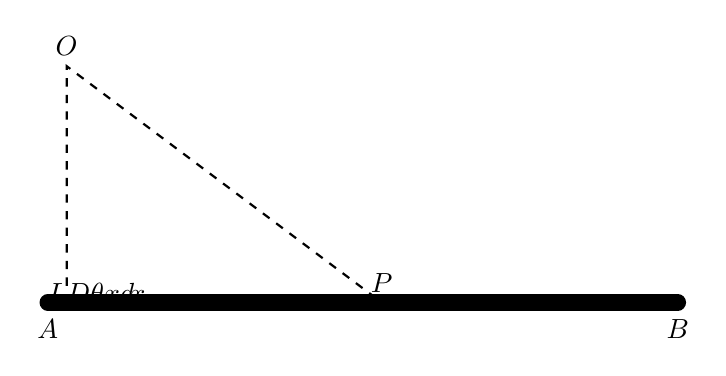
\begin{tikzpicture}
                \draw[line width=6,line cap=round] (0,0) node[below]{$A$}--(8,0) node[below]{$B$};
                \tzline[|<->|](0,-0.75)(8,-0.75){$L$}[mb]
                \draw[dashed,thick] (0,0)  coordinate (a)--(0,3) node[above]{$O$} coordinate (b) -- (4,0) node[above]{$P$} coordinate (c);
                % \draw (-0.2,0) to [dim arrow={label=$D$}] (-0.2,3);
                \tzline[|<->|](-0.5, 0)(-0.5, 3){$D$}[ml]
                \tzanglemark[->](a)(b)(c){$\theta$}[pos=1.5](15pt)
                \tzline[|->|, red](0, -1.5)(4, -1.5){$x$}[mb]
                \tzline[|->|, red](4, -1.5)(4.3, -1.5){$d\!x$}[mb]
            \end{tikzpicture}
        \end{center}
        \begin{solution}
            \addtolength{\jot}{2em}
            \begin{align*}
                \intertext{Consider a small element of length $d\!x$ at a distance $x$ from $A$.}\\
                \intertext{The mass of this element will be $d\!m$.}
                d\!m &= \lambda(\theta) d\!x\\
                \intertext{Relation between $x$ and $\theta$ can be found using $\tan\theta$.}
                \tan\theta &= \frac{x}{D}\\
                \intertext{Differentiating both sides with respect to $x$.}
                \sec^2\theta \frac{d\theta}{dx} &= \frac{1}{D}\\
                d\!x &= D \sec^2\theta d\theta\\
                \intertext{Substitute $d\!x$ in $d\!m$.}
                d\!m &= a\theta D \sec^2\theta d\theta\\
                \intertext{If we sum up the masses of all these elements, we get the mass of the rod.}
                m &= \int_{\textit{rod}} d\!m\\
                &= \int_0^{\tan^{-1}{\left(\frac{L}{D}\right)}} a\theta D \sec^2\theta d\theta\\
                &= aD \int_0^{\tan^{-1}{\left(\frac{L}{D}\right)}} \theta \sec^2\theta d\theta\\
                &= aD \left[\theta \tan\theta\right]_0^{\tan^{-1}{\left(\frac{L}{D}\right)}} - aD \int_0^{\tan^{-1}{\left(\frac{L}{D}\right)}} \tan\theta d\theta\\
                &= aD \left[\theta \tan\theta\right]_0^{\tan^{-1}{\left(\frac{L}{D}\right)}} + aD \left[\ln\left(\cos\theta\right)\right]_0^{\tan^{-1}{\left(\frac{L}{D}\right)}}\\
                &= aD \left[\tan^{-1}{\left(\frac{L}{D}\right)} \cdot \frac{L}{D} - 0\right] + aD \left[\ln\left(\cos\left(\tan^{-1}{\left(\frac{L}{D}\right)}\right)\right) - \ln\left(\cos 0\right)\right]\\
                &= aD \left[\tan^{-1}{\left(\frac{L}{D}\right)} \cdot \frac{L}{D}\right] + aD \left[\ln\left(\frac{D}{\sqrt{D^2+L^2}}\right)\right]\\
                \Aboxed{m &= aD \left[\tan^{-1}{\left(\frac{L}{D}\right)} \cdot \frac{L}{D} + \ln\left(\frac{D}{\sqrt{D^2+L^2}}\right)\right]}
            \end{align*}
        \end{solution}
        \BgThispage
\end{enumerate}

\pagebreak
\addcontentsline{toc}{section}{$\odot$}
\vspace*{\fill}
\begin{center}
    \begin{tikzpicture}
        \foreach \r in {0.2, 0.4, ..., 2}
        {
            \tzcircle(0, \r)(\r)
        }
    \end{tikzpicture}
\end{center}
\thispagestyle{empty}
\vspace*{\fill}